%! TeX program = lualatex
\documentclass[../main.tex]{subfiles}

\ifcsname preamble@file\endcsname
  \externaldocument[main-]{../../build/main}
  \setcounter{page}{\getpagerefnumber{main-week5}}
\fi

\begin{document} \makelectureweek{5}

\section{Power functions and \texorpdfstring{\(e^{x}\)}{exp(x)}}

Differentiation rules allows us to break up the task of differentiating a function into smaller and more manageable tasks.

\begin{mdframed}[style=simple]
  \textbf{Differentiation Rules} \hfill {\footnotesize (part \(1\) of \(4\))}
  \begin{align*}
    \frac{d}{dx} (c)
    &= 0, \text{ for any constant \(c\)}
    && \text{(constant)} \\[1em]
    \frac{d}{dx} (x^{n})
    &= n x^{n-1}, \text{ for any number \(n\), not just integers} 
    && \text{(power)} 
  \end{align*}

  Recall \(e\) is a special constant. We have a special derivative. 
  \[ 
    \frac{d}{dx} e^{x} = e^{x}.
  \]
\end{mdframed}

\faExclamationTriangle{} It is \emph{very important} that the power rule is applied to power functions, \emph{not} composite functions that look like power functions. Differentiating composite functions requires the chain rule! 

\begin{example}
  Evaluate \((x^{3})'\) and \(\frac{d}{dx}\frac{1}{\sqrt[3]{x}^{5}}\).
\end{example}
\vfill

\begin{example}
  Differentiate \(x^{e}\), \(x^{\pi}\), and \(e^{x}\).
\end{example}
\vfill

\begin{example}
  Can we directly apply the power rule to differentiate the following functions?
  \[
    \sqrt{-x^{2} + 1}, \qquad (4x^{2} + x - 1)^{2}, \qquad e^{-x}, \qquad e^{x^{2}}
  \]
\end{example}
\vspace{1cm}
\clearpage

\section{Addition, Subtraction and Constant Multiples}

\begin{mdframed}[style=simple]
  \textbf{Differentiation Rules} \hfill {\footnotesize (part \(2\) of \(4\))}

  If \(f\) and \(g\) are differentiable functions, then
  \begin{align*}
    \frac{d}{dx} [f(x) + g(x)] 
    &= \frac{d}{dx}f(x) + \frac{d}{dx}g(x)
    && \text{(sum)} \\[1em]
    \frac{d}{dx} [f(x) - g(x)] 
    &= \frac{d}{dx}f(x) - \frac{d}{dx}g(x)
    && \text{(difference)} \\[1em]
    \frac{d}{dx} [c f(x)] 
    &= c \, \frac{d}{dx} f(x), \text{ for any constant \(c\)}
    && \text{(constant multiple)}
  \end{align*}
\end{mdframed}

\textbf{Steps to calculate \(f'(x)\)}. 
\begin{enumerate}[label=(\arabic*)]
  \item Apply the \emph{sum} and \emph{difference} rules to the \emph{outermost} \(+\) and \(-\) in \(f(x)\). 
  \item Apply the constant multiple rule. 
\end{enumerate}
\bigskip

\begin{example}
  Differentiate \(2x^{2} + \sqrt{x} - 1\).
\end{example}
\vfill

\section{Products and Quotients}
\begin{mdframed}[style=simple]
  \textbf{Differentiation Rules} \hfill {\footnotesize (part \(3\) of \(4\))}

  If \(f\) and \(g\) are differentiable functions, then
  \begin{align*}
    \frac{d}{dx} [f(x)g(x)] 
    &= {g(x) \cdot \frac{d}{dx} [f(x)] + f(x) \cdot \frac{d}{dx}[g(x)]}
    && \text{(product)} \\
    &= g \cdot f' + f \cdot g' \\[1em]
    \frac{d}{dx} \frac{f(x)}{g(x)}
    &= {\frac{g(x) \cdot \frac{d}{dx} [f(x)] - f(x) \cdot \frac{d}{dx}[g(x)] }{ [g(x)]^{2} }}
    && \text{(quotient)} \\
    &= \frac{g \cdot f' - f \cdot g'}{g^{2}}
  \end{align*}
\end{mdframed}
\faExclamationTriangle{} Remember that \((fg)' \ne (f')(g')\) and \(\left(\frac{f}{g}\right)' \ne \frac{f'}{g'}\).

\textbf{Steps to calculate \(f'(x)\)}. 
\begin{enumerate}[label=(\arabic*)]
  \item Apply the \emph{sum} and \emph{difference} rules to the \emph{outermost} \(+\) and \(-\) in \(f(x)\). 
  \item Apply the \emph{constant multiple} rule.
  \item Apply the \emph{product} and \emph{quotient} rules.
\end{enumerate}
\bigskip

\begin{example}
  Differentiate \(xe^{x}\).
\end{example}
\vspace{1in}

\begin{example}
  Evaluate \(\frac{d}{dx} \frac{x^{\frac{3}{2}}}{\pi e^{x}}\).
\end{example}
\vfill
\clearpage

\begin{example}
  Differentiate \((x+2)\left( \frac{1}{x^{1/e}} - 1 \right)\).
\end{example}
\vfill
\clearpage

\begin{example}
  Differentiate \(e^{x}(2 \sqrt{x} - \sin(x))^{2}\).
\end{example}
\clearpage

\begin{example}
  Evaluate \(\frac{d}{dx} (4x^{2} + x - 1)^{2}\).
\end{example}
\vfill
\clearpage

\section{\texorpdfstring{\(\sin(x)\) and \(\cos(x)\)}{sin(x) and cos(x)}}
\begin{mdframed}[style=simple]
  Two more special derivatives.
  \[
    \frac{d}{dx} \sin(x) = \cos(x)
    \qquad
    \text{and}
    \qquad
    \frac{d}{dx} \cos(x) = -\sin(x)
  \]
\end{mdframed}
\bigskip

\begin{example}
  Find the fifth derivative of \(\sin(x)\).
\end{example}
\clearpage

\section{Three special limits and three proofs}
The number \(e\) is a special constant \emph{defined} as the solution to
\begin{equation} \label{eq:limit-exp}
  \lim_{h \to 0} \frac{e^{h} - 1}{h} = 1.
\end{equation}

\medskip
\begin{figure}[h!]  % [h] for here, [ht] for here top, [hb] for here bottom
  \centering
  \begin{tikzpicture}
    \tikzstyle{every node}=[font=\footnotesize];

    \begin{axis}[
      axis lines=middle,
      axis equal image,  % if true, must comment out width and height
      no markers,
      xtick={0}, ytick={0},
      enlargelimits=true, 
      ymax=2,
      ]
      \addplot[domain=-1:1] {e^x};
      \addplot[magenta, thick, domain=-1/2:1/2] {x + 1};
      \fill (axis cs:0,1) circle (2pt);
      \node[below left] at (axis cs:1/2,2) {\(e^{x}\)};
    \end{axis}
  \end{tikzpicture}
\end{figure}

\textbf{Theorem}. 
\[
  \frac{d}{dx} e^{x} = e^{x}.
\]

\bigskip
\textbf{Proof}. 

\vfill

The Squeeze Theorem allows us to calculate two special limits. See page 195 of the textbook.
\begin{equation} \label{eq:limits-trigs}
  \lim_{h \to 0} \frac{\sin(h)}{h} = 1
  \qquad\text{and}\qquad
  \lim_{h \to 0} \frac{\cos(h) - 1}{h} = 0
\end{equation}

\medskip
\begin{figure}[h!]
  \centering
  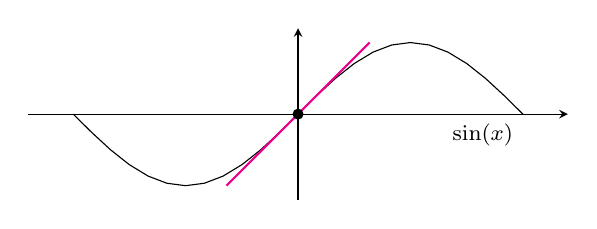
\begin{tikzpicture}
    \tikzstyle{every node}=[font=\footnotesize];

    \begin{axis}[
      axis lines=middle,
      axis equal image,  % if true, must comment out width and height
      no markers,
      xtick={0}, ytick={0},
      enlargelimits=true, 
      ]
      \addplot[domain=-pi:pi] { sin(deg(x)) };
      \addplot[magenta, thick] coordinates { (-1,-1) (1,1) };
      \fill (axis cs:0,0) circle (2pt);
      \node[below left] at (axis cs:pi,0) {\(\sin(x)\)};
    \end{axis}
  \end{tikzpicture}
  \qquad
  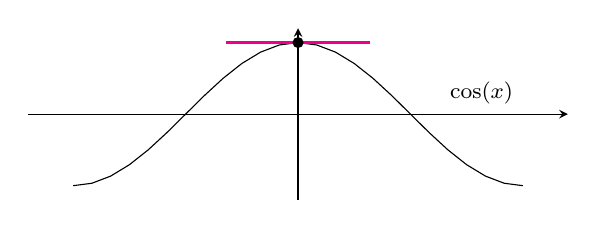
\begin{tikzpicture}
    \tikzstyle{every node}=[font=\footnotesize];

    \begin{axis}[
      axis lines=middle,
      axis equal image,  % if true, must comment out width and height
      no markers,
      xtick={0}, ytick={0},
      enlargelimits=true, 
      ]
      \addplot[domain=-pi:pi] { cos(deg(x)) };
      \addplot[magenta, thick] coordinates { (-1,1) (1,1) };
      \fill (axis cs:0,1) circle (2pt);
      \node[above left] at (axis cs:pi,0) {\(\cos(x)\)};
    \end{axis}
  \end{tikzpicture}
\end{figure}

\clearpage
\textbf{Theorem}. 
\[
  \frac{d}{dx} \sin(x) = \cos(x).
\]

\textbf{Idea}. Use the \emph{definition of the derivative} (as a function) and the sine addition formula
\begin{equation} \label{eq:sin-addition}
  \sin(x + h) = \sin(x) \cos(h) + \cos(x) \sin(h).
\end{equation}
Try to take advantage of the special limits in Equations~\eqref{eq:limits-trigs}.

\bigskip
\textbf{Proof}.
\clearpage

\textbf{Theorem}. 
\[
  \frac{d}{dx} \cos(x) = -\sin(x).
\]

\textbf{Idea}. Use the \emph{definition of the derivative} (as a function) and the cosine addition formula
\begin{equation} \label{eq:cos-addition}
  \cos(x + h) = \cos(x) \cos(h) - \sin(x) \sin(h).
\end{equation}
Try to take advantage of the special limits in Equations~\eqref{eq:limits-trigs}.

\bigskip
\textbf{Proof}.  
\clearpage

\section{The Chain Rule}
\begin{mdframed}[style=simple]
  \textbf{Differentiation Rules} \hfill {\footnotesize (part \(4\) of \(4\))}

  If \(g\) is differentiable at \(x\) and \(f\) is differentiable at \(g(x)\), then the composite function \(F = f \circ g\) defined by \(F(x) = f(g(x))\) is differentiable at \(x\) and \(F'\) is given by 
  \begin{align*}
    \frac{d}{dx} F(x) 
    &= f'(g(x)) g'(x)
    &&\text{(the chain rule)}\\[1em]
    &= \frac{dy}{du} \frac{du}{dx}, \text{ if we write } y = f(u), u = g(x).
  \end{align*}
\end{mdframed}

\textbf{Steps to calculate \(f'(x)\)}.
\begin{enumerate}[label=(\arabic*)]
  \item Apply the \emph{sum} and \emph{difference} rules to the \emph{outermost} \(+\) and \(-\) in \(f(x)\). 
  \item Apply the \emph{constant multiple} rule.
  \item Apply the \emph{product}, the \emph{quotient}, or the \emph{chain} rule. We might be able to simplify a calculation if we group certain terms together. 
\end{enumerate}
\bigskip

\begin{example}
  Differentiate \((x+1)^{3}\).
\end{example}


\clearpage

\begin{example}
  Differentiate \(e^{x}(2\sqrt{x} - \sin(x))^{2}\).
\end{example}
\clearpage

\section{In-class exercises}
Explore differentiation techniques and reflect on your methods. Discuss your \emph{methods} with others. What \emph{skills} do you find helpful? How do you \emph{organize} your calculation? What can you \emph{learn} from others?

More space is provided starting on the next page.

\bigskip
\begin{example}
  Let \(f(x) = x^{5} + x^{4} + x^{3} + x^{2} + x^{1} + 1\). What is \(f^{(6)}\)?
\end{example}

\bigskip
\begin{example}
  Is there a \emph{positive} integer \(n\) such that \(\frac{d^{n}}{dx^{n}} \left( x^{-1} \right) = 0\)? If so, find such integer. If not, explain why such integer does not exist.
\end{example}

\bigskip

\begin{example}
  Suppose \(f\) is a function that satisfy \(f'(x) = f'(0) f(x)\). Find \(f'', f'''\). What is \(f^{(99)}\)?
\end{example}

\bigskip
\begin{example}
  Find \emph{two} different methods to differentiate \(x^{3} + 3x^{2} + 3x + 3\).
\end{example}

\bigskip
\begin{example}
  Differentiate \(\tan(x)\). 
\end{example}

\bigskip
\begin{example}
  Differentiate \(\tan(x)^{3} + 3 \sec(x)^{2} + 3\tan(x)\). 
\end{example}

\bigskip
\begin{example}
  Differentiate \(x^{1/2} e^{x} \sqrt{\cos(x)^{2} + 5}\).
\end{example}
\bigskip

\clearpage
\setcounter{thm}{2}
\begin{example}
  Let \(f(x) = x^{5} + x^{4} + x^{3} + x^{2} + x^{1} + 1\). What is \(f^{(6)}\)?
\end{example}
\vfill

\begin{example}
  Is there a \emph{positive} integer \(n\) such that \(\frac{d^{n}}{dx^{n}} \left( x^{-1} \right) = 0\)? If so, find such integer. If not, explain why such integer does not exist.
\end{example}
\vfill

\begin{example}
  Suppose \(f\) is a function that satisfy \(f'(x) = f'(0) f(x)\). Find \(f'', f'''\). What is \(f^{(99)}\)?
\end{example}
\vfill

\clearpage
\begin{example}
  Find \emph{two} different methods to differentiate \(x^{3} + 3x^{2} + 3x + 3\).
\end{example}
\vspace{2in}

\bigskip
\begin{example}
  Differentiate \(\tan(x)\). 
\end{example}

\vspace{3in}
\begin{example}
  Differentiate \(\tan(x)^{3} + 3 \sec(x)^{2} + 3\tan(x)\). 
\end{example}
\clearpage

\begin{example}
  Differentiate \(x^{1/2} e^{x} \sqrt{\cos(x)^{2} + 5}\).
\end{example}
\end{document}
